%%
%% This is file `sample-sigplan.tex',
%% generated with the docstrip utility.
%%
%% The original source files were:
%%
%% samples.dtx  (with options: `sigplan')
%% 
%% IMPORTANT NOTICE:
%% 
%% For the copyright see the source file.
%% 
%% Any modified versions of this file must be renamed
%% with new filenames distinct from sample-sigplan.tex.
%% 
%% For distribution of the original source see the terms
%% for copying and modification in the file samples.dtx.
%% 
%% This generated file may be distributed as long as the
%% original source files, as listed above, are part of the
%% same distribution. (The sources need not necessarily be
%% in the same archive or directory.)
%%
%%
%% Commands for TeXCount
%TC:macro \cite [option:text,text]
%TC:macro \citep [option:text,text]
%TC:macro \citet [option:text,text]
%TC:envir table 0 1
%TC:envir table* 0 1
%TC:envir tabular [ignore] word
%TC:envir displaymath 0 word
%TC:envir math 0 word
%TC:envir comment 0 0
%%
%%
%% The first command in your LaTeX source must be the \documentclass command.
\documentclass[sigplan,anonymous,review]{acmart}

%%
%% \BibTeX command to typeset BibTeX logo in the docs
\AtBeginDocument{%
  \providecommand\BibTeX{{%
    Bib\TeX}}}

%% Rights management information.  This information is sent to you
%% when you complete the rights form.  These commands have SAMPLE
%% values in them; it is your responsibility as an author to replace
%% the commands and values with those provided to you when you
%% complete the rights form.
\setcopyright{acmcopyright}
\copyrightyear{2018}
\acmYear{2018}
\acmDOI{XXXXXXX.XXXXXXX}

%% These commands are for a PROCEEDINGS abstract or paper.
\acmConference[Conference acronym 'XX]{Make sure to enter the correct
  conference title from your rights confirmation emai}{June 03--05,
  2018}{Woodstock, NY}
\acmPrice{15.00}
\acmISBN{978-1-4503-XXXX-X/18/06}


%%
%% Submission ID.
%% Use this when submitting an article to a sponsored event. You'll
%% receive a unique submission ID from the organizers
%% of the event, and this ID should be used as the parameter to this command.
%%\acmSubmissionID{123-A56-BU3}

%%
%% For managing citations, it is recommended to use bibliography
%% files in BibTeX format.
%%
%% You can then either use BibTeX with the ACM-Reference-Format style,
%% or BibLaTeX with the acmnumeric or acmauthoryear sytles, that include
%% support for advanced citation of software artefact from the
%% biblatex-software package, also separately available on CTAN.
%%
%% Look at the sample-*-biblatex.tex files for templates showcasing
%% the biblatex styles.
%%

%%
%% The majority of ACM publications use numbered citations and
%% references.  The command \citestyle{authoryear} switches to the
%% "author year" style.
%%
%% If you are preparing content for an event
%% sponsored by ACM SIGGRAPH, you must use the "author year" style of
%% citations and references.
%% Uncommenting
%% the next command will enable that style.
%%\citestyle{acmauthoryear}

\usepackage{booktabs, multirow} % for borders and merged ranges
\usepackage{soul}% for underlines
\usepackage{comment}
%A set of custom commands that are used for my personal latex style
%Created: Feb 2020
%Updated: July 2020
\usepackage{listings}

\newcommand{\defn}[1]{\textbf{#1}} %definitions are bold
\newcommand{\jnote}[1]{\textcolor{blue}{Justin: #1\\}} %a note from Justin
\newcommand{\rnote}[1]{\textcolor{orange}{Ron: #1\\}} %a note from Ron
\newcommand{\pnote}[1]{\textcolor{purple}{Peyton: #1\\}} %a note from Peyton
\newcommand{\todo}[1]{\textcolor{red}{TODO: #1\\}} %a todo note

\definecolor{tangerine}{RGB}{245,166,35} %comments, primary color
\definecolor{blueSeaFoam}{RGB}{80,227,194}
\definecolor{liteGreen}{RGB}{184,233,134 }
\definecolor{royalBlue}{RGB}{74,144,226} %keywords
\definecolor{amaranth}{rgb}{0.9, 0.17, 0.31} %special keywords
\definecolor{lavender}{rgb}{0.71, 0.49, 0.86}

\lstdefinestyle{mystyle}{
    backgroundcolor=\color{white},   
    commentstyle=\color{tangerine},
    keywordstyle=\color{royalBlue},
    identifierstyle=\color{black},
    numberstyle=\tiny\color{gray},
    basicstyle=\ttfamily\footnotesize,
    breakatwhitespace=false,         
    breaklines=true,                 
    captionpos=b,                    
    keepspaces=true,                 
    numbers=left,                    
    numbersep=5pt,                  
    showspaces=false,                
    showstringspaces=false,
    showtabs=false,                  
    tabsize=2,
    frame=lines,
    %just for Chisel
    emph={Module, IO, Input, Output, UInt, Bool, Wire, Vec, before, after, extend, in, register, insert, apply, Pointcutter, AfterToken},
    emphstyle=\color{amaranth}
}

\lstset{style=mystyle}
\raggedbottom


%%
%% end of the preamble, start of the body of the document source.
\begin{document}

%%
%% The "title" command has an optional parameter,
%% allowing the author to define a "short title" to be used in page headers.
\title{Foam: Feature-Oriented Construction of Finite State Machines}

%%
%% The "author" command and its associated commands are used to define
%% the authors and their affiliations.
%% Of note is the shared affiliation of the first two authors, and the
%% "authornote" and "authornotemark" commands
%% used to denote shared contribution to the research.
\author{Ben Trovato}
\authornote{Both authors contributed equally to this research.}
\email{trovato@corporation.com}
\orcid{1234-5678-9012}
\author{G.K.M. Tobin}
\authornotemark[1]
\email{webmaster@marysville-ohio.com}
\affiliation{%
  \institution{Institute for Clarity in Documentation}
  \streetaddress{P.O. Box 1212}
  \city{Dublin}
  \state{Ohio}
  \country{USA}
  \postcode{43017-6221}
}

\author{Lars Th{\o}rv{\"a}ld}
\affiliation{%
  \institution{The Th{\o}rv{\"a}ld Group}
  \streetaddress{1 Th{\o}rv{\"a}ld Circle}
  \city{Hekla}
  \country{Iceland}}
\email{larst@affiliation.org}

\author{Valerie B\'eranger}
\affiliation{%
  \institution{Inria Paris-Rocquencourt}
  \city{Rocquencourt}
  \country{France}
}

\author{Aparna Patel}
\affiliation{%
 \institution{Rajiv Gandhi University}
 \streetaddress{Rono-Hills}
 \city{Doimukh}
 \state{Arunachal Pradesh}
 \country{India}}

\author{Huifen Chan}
\affiliation{%
  \institution{Tsinghua University}
  \streetaddress{30 Shuangqing Rd}
  \city{Haidian Qu}
  \state{Beijing Shi}
  \country{China}}

\author{Charles Palmer}
\affiliation{%
  \institution{Palmer Research Laboratories}
  \streetaddress{8600 Datapoint Drive}
  \city{San Antonio}
  \state{Texas}
  \country{USA}
  \postcode{78229}}
\email{cpalmer@prl.com}

\author{John Smith}
\affiliation{%
  \institution{The Th{\o}rv{\"a}ld Group}
  \streetaddress{1 Th{\o}rv{\"a}ld Circle}
  \city{Hekla}
  \country{Iceland}}
\email{jsmith@affiliation.org}

\author{Julius P. Kumquat}
\affiliation{%
  \institution{The Kumquat Consortium}
  \city{New York}
  \country{USA}}
\email{jpkumquat@consortium.net}

%%
%% By default, the full list of authors will be used in the page
%% headers. Often, this list is too long, and will overlap
%% other information printed in the page headers. This command allows
%% the author to define a more concise list
%% of authors' names for this purpose.
\renewcommand{\shortauthors}{Trovato et al.}

%%
%% The abstract is a short summary of the work to be presented in the
%% article.
\begin{abstract}
  Finite-State Machines are really cool.
\end{abstract}

%%
%% The code below is generated by the tool at http://dl.acm.org/ccs.cfm.
%% Please copy and paste the code instead of the example below.
%%
\begin{CCSXML}
<ccs2012>
<concept>
<concept_id>10011007.10011006.10011041.10011047</concept_id>
<concept_desc>Software and its engineering~Source code generation</concept_desc>
<concept_significance>500</concept_significance>
</concept>
<concept>
<concept_id>10010583.10010682.10010689</concept_id>
<concept_desc>Hardware~Hardware description languages and compilation</concept_desc>
<concept_significance>500</concept_significance>
</concept>
</ccs2012>
\end{CCSXML}

\ccsdesc[500]{Software and its engineering~Source code generation}
\ccsdesc[500]{Hardware~Hardware description languages and compilation}

%%
%% Keywords. The author(s) should pick words that accurately describe
%% the work being presented. Separate the keywords with commas.
\keywords{feature-oriented programming, finite state machines, generative programming, hardware generation}
%% A "teaser" image appears between the author and affiliation
%% information and the body of the document, and typically spans the
%% page.

%%
%% This command processes the author and affiliation and title
%% information and builds the first part of the formatted document.
\maketitle

\section{Introduction}

The advent of hardware-generation languages~\cite{hwgen} has promoted the adoption of techniques and abstractions by hardware designers that were previously available only to software systems and their designers.   Hardware-characterization languages such as VHDL~\cite{vhdl} and Verilog~\cite{verilog} describe the components and interconnections of hardware circuit elements, much like HTML describes the components and references of a web page.  While those languages provide some abstractions (such as arithmetic operations and restrictive macros), the paradigms and practices used widely in successful software engineering efforts are largely unavailable.

By contrast, hardware-generation approaches allow a designer to write a program, and the output of that program's execution is the hardware design.  The program can be authored using paradigms that promote efficient software construction, reuse, rigorous testing, and clarity of expression.  Our work in this paper builds on the hardware-generation language Chisel~\cite{chisel:book}, which is in turn built on Scala~\cite{scala-overview-tech-report}.   Chisel is essentially a Scala library that generates Verilog when a hardware design is executed.

A simple and recent example showing the advantages of hardware generation over characterization concerns an adder~\cite{Deters:adder}.   Using VHDL, a hardware designer can request that an adder circuit be optimized for either for delay (carry lookahead) or for area (carry propagate).   Using Chisel, an adder can be specified that combines both forms of carry computation, to meet a timing or area constraint while otherwise optimized in the other dimension.

Chisel has also proven itself robust in pedagogy and industry, serving as the basis for courses in digital logic~\cite{vlsicourse} and serving as a platform for describing RISC-V systems~\cite{chisel:riscv}.  Our long-term goal \pnote{What is our long-term goal?}

In this paper, we consider a feature-oriented approach to generating hardware, specifically finite state machines. A given feature can affect multiple regions of a finite state machine.  For example, the cache system  we consider in Section~\ref{sec:cache} could use write-back or write-through in response to a store operation.  Expressed as a feature, write-back affects both the store operation (marking the line dirty) and the fetch operation (causing dirty lines to be written to the backing store on eviction).  Aspect-oriented programming (AOP)~\cite{aop} is a paradigm well suited to expression of cross-cutting concerns that affect multiple regions of software systems.  For example, AspectJ~\cite{aspectj} allows expression of advice that is applied at prescribed join points of a software system written in Java.  While our thinking is aspectual in terms of formulating a feature-oriented approach to finite state machines, we are fortunate that hardware generation languages such as Chisel suffice to express the requisite transformations:  no new language is needed.

In Section~\ref{sec:prior} we summarize feature-oriented approaches for software systems and other inspirations for our work.  As compared with monolithic designs, feature-oriented systems omit unnecessary code, resulting in smaller footprint and higher throughput.
Sections~\ref{sec:decomp} and~\ref{sec:formal} describe a feature-oriented approach for generating finite state machines using two complementary techniques.  We illustrate those techniques separately on the examples of a vending machine (Section~\ref{sec:vend}) and the game of Nim (Section~\ref{sec:nim}). In Section~\ref{sec:cache}, the techniques are then applied in concert to generate a multiprocessor cache with a simple coherence protocol.

\section{Prior Work}\label{sec:prior}

Our work builds on a programming paradigm available in the software community that efficiently supports the expression and application of \emph{cross-cutting} concerns in a software system.  Aspect-Oriented Programming~(AOP)~\cite{Kicz97} and its realization in systems such as AspectJ~\cite{aspectj} allow developers to express ideas in a software system that affect multiple components of that system in support of a common idea or feature.   A commonly cited example is the implementation of a logging feature, so that every method when called and prior to returning logs those events to some output stream.   Absent an AOP approach, a developer is faced with the following difficulties:
\begin{itemize}
    \item Implementation of the feature would require modifying every method at its entry and every possible exit so that it emitted the proper log messages.  This is both tedious and error-prone, especially if methods can exit due to unforeseen actions such as exceptions.
    \item Removing the feature, should it no longer be needed, is also tedious and error-prone.
    \item Placing the feature under some kind of conditional execution offers some relief, but
    \begin{itemize}
        \item The conditions themselves incur execution time and the logging code occupies code space.
        \item Subsequent modifications to the system must be mindful to include properly the logging actions.
    \end{itemize}
\end{itemize}
Macro processors can achieve the proper effect, namely including the code only when it is desired.  However, it is still incumbent on developers to remember to call the macros at the proper points in a program.

AOP is the perfect solution to this and similar problems, because a developer can specify that at \emph{every} method entry and exit (other than the method that does the logging), a segment of code should be inserted to accomplish the appropriate logging.  If the logging is no longer desired, the associated aspect is simply omitted when building the system.  In this way, both originally and upon modification, all methods' entries and exits are properly logged.

Feature-Oriented Programming~(FOP)~\cite{prehofer1997feature} builds on this idea by expressing features in an aspectual manner.   Expressed in this manner, a feature is essentially a recipe for rewriting a software system to implement the feature.   The common example given for this paradigm is that of a \emph{cache}, say in a web browser.  Where the browser would normally issue a request to a web site on behalf of a given URL (which could take some time), the cache feature would first check if the browser had recently fetched that URL, satisfying the request with the cached information. Implementation of this feature requires storage to hold previously fetched information, code to manage that storage, and a rewrite of the base system to cause the cache to be consulted prior to issuing the web request.  Expressed aspectually, a cache could be imposed throughout the browser, in any situation where such a web request could be made.

The feature on its own is insufficient to realize any benefits.  The software system must be written in such a way to accept the feature. As more features are conceived and implemented, the base system and any extant features may require revision.   In the end, a system is obtained where orthogonal features compose effortlessly, in any combination, to realize a desired subset of all possible features.

This approach to creating featureful systems has the empirical advantages described below. This approach has also been attractive for managing product lines in which features evolve over time, affecting not only the base system but also other features~\cite{10.1145/2897695.2897701}.

An example that has been treated with this approach is the CORBA~\cite{} Event Channel~\cite{}.  The standard implementation is \emph{monolithic}, offering all possible features in all allowable combinations.    
When expressed in terms of composable features, the 

\section{Running Example: Vending Machine}
\subsection{Vending Machine}\label{sec:vend}
We will utilize a vending machine as a motivating example in the following sections. A vending machine is an apt example for our technique as it not only has a complex internal state (it must keep track of the amount of money inserted, which product to dispense, etc), but also many different features that could be required. Below we have listed features one might find. Figure~\ref{fig:vmDependencies} shows the dependencies between all the features in the vending machine.

\begin{itemize}
    \item Add Currency: Admit a token of currency of any arbitrary denomination and arbitrary number of times to an arbitrary value threshold.
    \item Dispense Product: Dispense a product if the value of the product has been inserted and the button pressed.
    \item Print Funds: After a coin is inserted into the vending machine, display the total funds.
    \item Insufficient Funds: After a product button is pushed, if there is an insufficient amount of funds, display this warning.
    \item Change Return: Push the change return button and get your coins back.
    \item Peanut Warning: Before a product that contains nuts can be purchased, the customer has to confirm this decision.
    \item Buy More: Allow the customer to buy as many products as they want until the value in the machine reaches zero.
\end{itemize}

\begin{figure}[htbp]
    \centering
    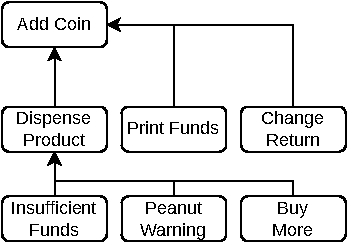
\includegraphics{figures/VendingMachine.pdf}
    \caption{Dependencies between vending machine features.}
    \label{fig:vmDependencies}
\end{figure}

\section{Feature Decomposition}\label{sec:decomp}
\jnote{Do we need to talk about abstract and concrete features here or just point people to prior work?}
\subsection{Cross-Cutting Features}

\subsection{Cross Product Features}

\section{Formalism}\label{sec:formal}
We have developed formalisms to describe each of the feature decomposition techniques. Following from the classical definition of finite state machines $M = (Q, \Sigma, \delta, q_0, F)$, $Q$ is a set of states, $\Sigma$ is a set of input symbols, $\delta$ is the transition function, $q_0$ is the start state, and $F$ is the set of accepting states. \\

\subsection{Cross Cutting Features}
Any path through the FSM can be described as a sequence of alternating states and input tokens. For example, the FSM in Figure~\ref{fig:example} contains two paths from the start to accept state: $XxYyZ$ and $XtZ$. When we apply features to the FSM we change the paths through the machine, thus also changing the accepted language.

\begin{figure}[htb]
    \centering
    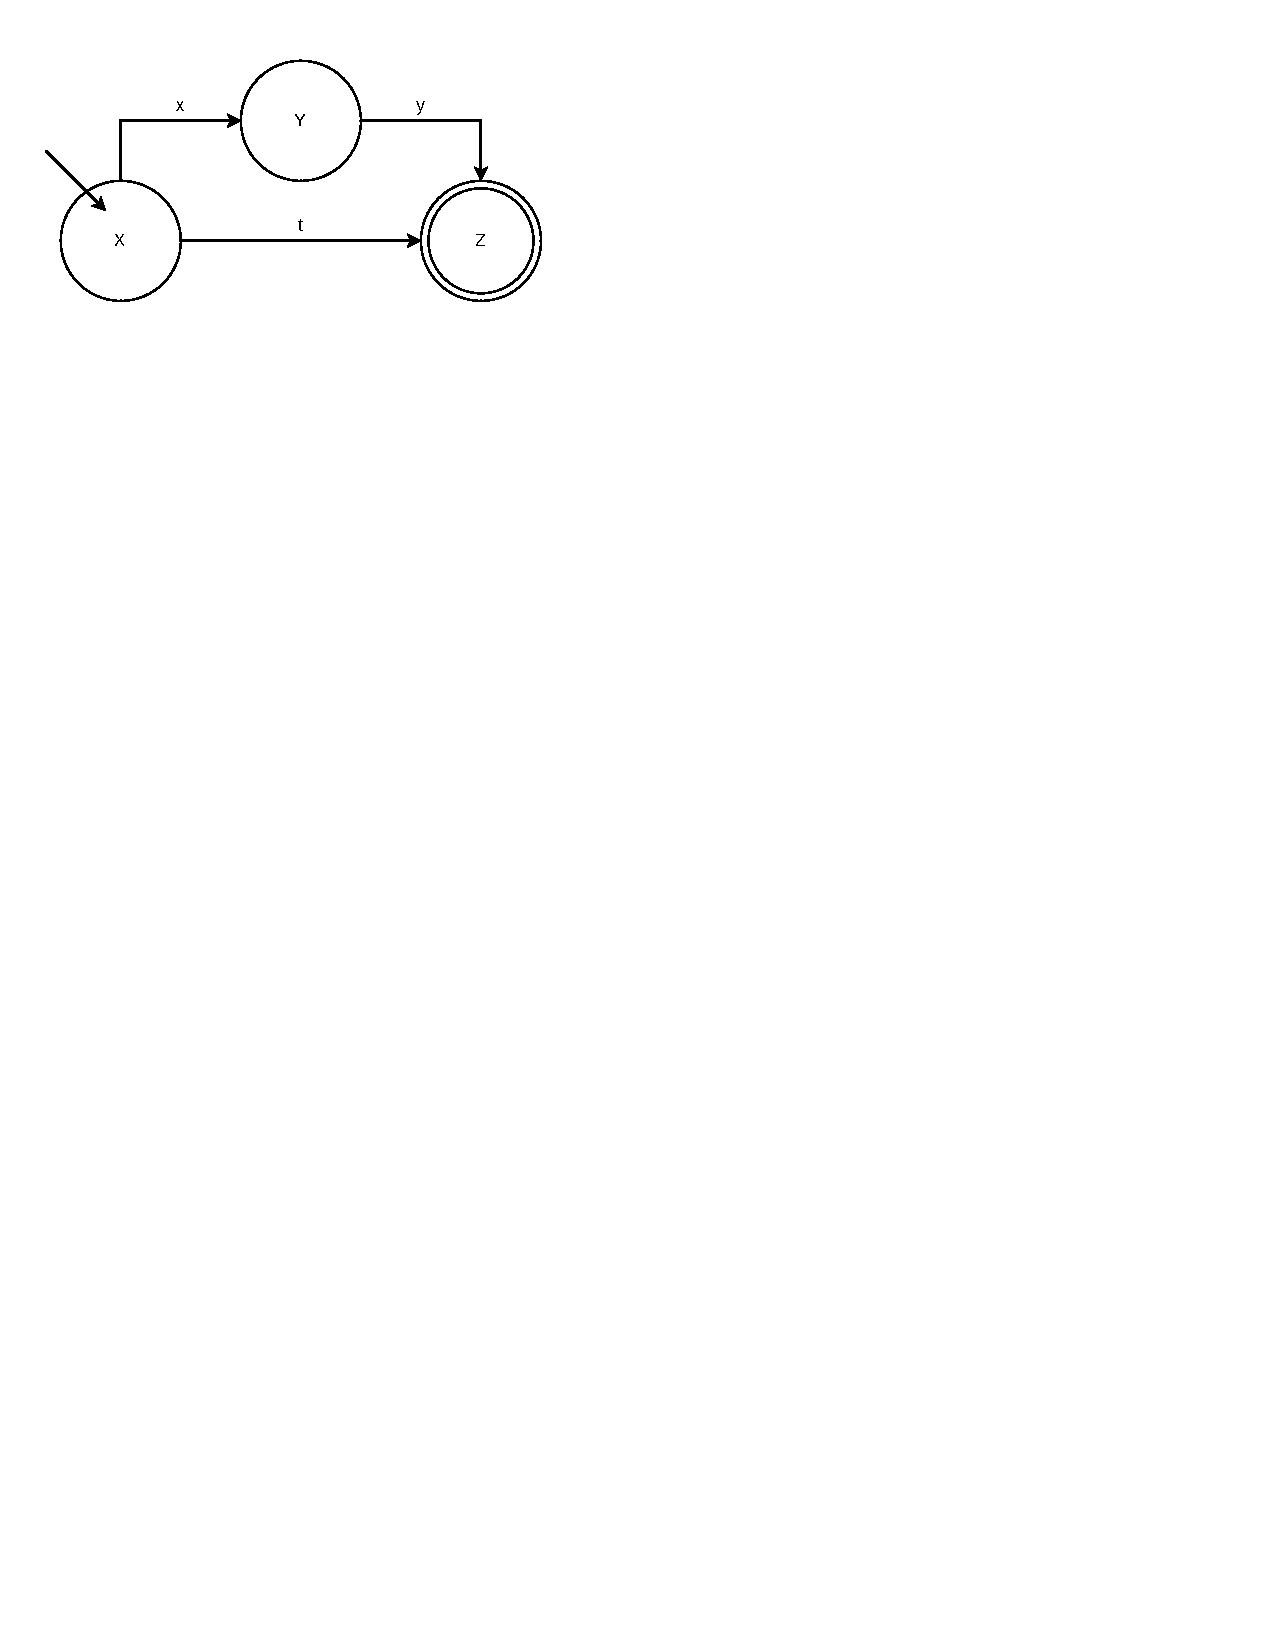
\includegraphics{figures/ExampleFSM.pdf}
    \caption{Example FSM}
    \label{fig:example}
\end{figure}

\paragraph{Pointcuts} Before applying advice, we must define where in the FSM the advice will be. We define both pointcuts for both states and input tokens. As such, a pointcut $\Pi$ is either $\Pi = \{q : q \in Q, C(q) = \mathrm{true}\}$ or $\Pi = \{\sigma : \sigma \in \Sigma, C(\sigma) = \mathrm{true}\}$, where $C$ is some matching criteria such as type.

\paragraph{Advice} In our formalism, advice $\Delta$ is a function that returns a valid path through the FSM. These paths may be arbitrary in length\footnote{In our implementation, we only allow paths of length two. Simply, we have not run into a situation where a longer one is necessary, but there is no technical limitation on path length.}. The pattern of the required path depends on where in the FSM the pointcut is making modifications. Since a state may have multiple paths go through it or an input token may be used in multiple paths, $\Delta$ is not parameterized with the join-point $p$, but also information about the path it is being applied to. Advice in our system is \emph{context aware}, meaning that $\Delta$ can return different paths depending upon the path under consideration. 

For simplicity, we introduce three sets of path information $\Theta, \Omega$, and $\Gamma$ defined as:
\begin{align*}
    \Theta &= \{A \alpha | \forall p \in \Pi \ p \in \delta(A, \alpha)\}\\
    \Omega &= \{\beta B | \forall p \in \Pi \ B \in \delta(p, \beta)\}\\
    \Gamma &= \{AB | \forall p \in \Pi \ \forall A \in \Sigma \ \forall B \in \delta(A, p)\}
\end{align*}

$\Theta$ and $\Gamma$ capture all the immediate paths that the state join-point $p$ is involved in. Whereas, $\Gamma$ captures the paths that the transition join-point $p$ is involved in. 

\subsubsection{State Features}
We can now express the three types of advice application for states in terms of $\Pi, \Delta, \Theta$, and $\Omega$.\\
\textbf{Before:} $\forall p \in \Pi \ \forall A \alpha \in \Theta \quad A \alpha p \rightarrow A \alpha \Delta(p, A \alpha)p$\\
\textbf{After:} $\forall p \in \Pi \ \forall \beta B \in \Omega \quad p\beta B \rightarrow P\Delta(p, \beta B)\beta B$\\
\textbf{Around:} \\
$\forall p \in \Pi \ \forall A \alpha \in \Theta \ \forall \beta B \in \Omega \quad A \alpha p \beta B \rightarrow A \alpha \Delta(p, A \alpha, B \beta) \beta B $
\paragraph{Buy More} As an example, let's consider the \textbf{Buy More} feature. After each time the machine despenses a product (represented in the system as a \texttt{DispenseState}) the machine should transition back to a state where the total value in the machine represents product price subtracted from the original value in the machine (represented as a \texttt{TotalState}).

\begin{align*}
    \Pi & \text{ where } C = \{p.\mathrm{type} = \mathrm{DispenseState}\}\\
    \Delta &= \{\\
    &\mathrm{funds} \leftarrow p.\mathrm{value} - p.\mathrm{product.value}\\
    &\mathrm{return} (\lambda, \mathrm{TotalState(funds)})\\
    \}\\
    &\mathrm{Around}(\Pi, \Delta)
\end{align*}

\subsubsection{Transition Features}
Similarly we can express the three types of advice application for input tokens in terms of $\Pi, \Delta$, and $\Gamma$.\\
\textbf{Before:} $\forall p \in \Pi \ \forall AB \in \Gamma \quad A p B \rightarrow A \Delta(p, A, B)pB$\\
\textbf{After:} $\forall p \in \Pi \ \forall AB \in \Gamma \quad A p B \rightarrow A p \Delta(p, A, B)B$\\
\textbf{Around:} $\forall p \in \Pi \ \forall AB \in \Gamma \quad A p B \rightarrow A  \Delta(p, A, B)B$

\paragraph{Print Funds} For an example of applying advice to an input token, let's consider the \textbf{Print Funds} feature. Here, after each transition on a piece of currency, the machine should print out the new total value. Note, here we need to check the value of $B$ to make sure that we do not reapply the same advice again.

\begin{align*}
    \Pi & \text{ where } C = \{p.\mathrm{type} = \mathrm{CurrencyToken}\}\\
    \Delta &= \{\\
    &\mathrm{newState} \leftarrow \mathrm{PrinterState(} B.\mathrm{value})\\
    &\text{if } B = \mathrm{newState} \text{ return } (\mathrm{None})\\
    &\text{else return} (\mathrm{newState}, \lambda)\\
    \}\\
    &\mathrm{After}(\Pi, \Delta)
\end{align*}

\subsection{Cross Product Features}
\pnote{Do we provide motivation here? E.g., how this is different from the union/intersection machine constructs, and how this is fundamentally different from the concatenation machine?}
\pnote{Where should we reference Sipser's proof of regular languages being closed under union?}

Let $M_1 = (Q_1, \Sigma_1, \delta_1, q_{01}, F_1)$ and $M_2 = (Q_2, \Sigma_2, \delta_2, q_{02}, F_2)$ be finite state machines. Then we may construct the cross product machine, $M = M_1 \times M_2 = (Q, \Sigma, \delta, q_0, F)$ as: 

\begin{enumerate}
    \item $Q = Q_1 \times Q_2$
    \item $\Sigma = \Sigma_1 \times \Sigma_2$
    \item $q_0 = (q_{01}, q_{02})$
    \item $F = (F_1 \times Q_2) \cap (Q_1 \times F_2)$
    \item Define $\delta$ such that $\forall \mathbf{r} = (r_1, r_2) \in Q, \forall \mathbf{a} = (a_1, a_2) \in \Sigma,$ 
\end{enumerate}
\[\delta(\mathbf r, \mathbf a) = \begin{cases}
    (\delta_1(r_1, a_1), \delta_2(r_2, a_2)) & \delta_i(r_i, a_i) \neq \emptyset, i = 1, 2\\
    \emptyset & \mathrm{else}
\end{cases}\]


\section{Foam: Aspect Oriented Finite State Machine Library}
We have implemented an aspect oriented finite state machine library, which we call Foam,  in Scala\footnote{https://github.com/wustl-frisc/foam}. In this section we detail the programmer interface as well as how the library generates usable source code. Following our vending machine example, Figure \ref{lst:PrintFunds} shows the implmentation of the \textbf{Print Funds} feature in Foam.

\subsection{Interface}
While Foam is not a fully fledged domain specific language, we have modeled the interface after the well established aspect-oriented extension to Java, AspectJ~\cite{}. The intention is to give aspect-oriented practitioners a familiar interface for interacting with the finite state machines. Since the library is implemented in plain Scala we have access to and utilize the full powers of the type system. 

The base classes in Foam are \texttt{NFA}, \texttt{State}, and \texttt{Token}. From these three classes programmers can extend their functionality with any implementation information they need. All features are applied to the \texttt{NFA} class. This class has a single public facing function \texttt{addTransition((State, Token), State)}.

We provide an \texttt{Aspect} class that contains all the mechanisms to create aspects. Any number of pointcuts and advice can be defined within a single aspect. Since this is a plain Scala class, aspects can also call other aspects and be nested at the programmer's discretion for code reuse.

\paragraph{Pointcuts} Just as in AspectJ, we have decoupled the creation of pointcuts from the implementation of advice. The \texttt{Pointcutter} object allows programmers to collect join-points by matching on their defined criteria. Pointcuts in our system are simply sets of \texttt{State} or \texttt{Token} objects. The \texttt{Pointcutter} automatically casts the objects to subtypes via type parameterization. Figure \ref{lst:PrintFunds} shows the construction of a \texttt{Token} pointcut on lines 4-7.

\paragraph{Advice} Foam has before, after, and around advice that comes in both state and token flavors. Advice is implemented by passing an anonymous function to the advice object. Following the formalism in Section \ref{sec:formal}, the implementation must return a path through the finite state machine. Note, in our implmentation we have chosen to only allow paths of lenght two. However, longer paths are possible with changes to the library. Since this is just a simple Scala function, any other legal Scala code may be used in the implementation. 

Again, following the formalism from Section \ref{sec:formal}, the advice implementation is executed for each path that the join-point might be involved in. To make this easy for the user, we take a cue from AspectJ and provide reflective access to the join-point through the \texttt{thisJoinpoint} parameter. \texttt{thisJoinpoint.point} gives direct access to the object the join-point represents. \texttt{thisJoinpoint.in} represents the currently executed path into the join-point. \texttt{thisJoinpoint.out} represents the currently executed path out of the join-point. Lines 9-15 demonstrate how this is all used together to implement advice for the \textbf{Print Funds} feature.

\begin{figure*}[h]
    \centering
    \begin{lstlisting}[language = Scala]
class PrintFunds extends Aspect[NFA] {
  def apply(nfa: NFA) = {

    val tokenPointcut = Pointcutter[Token, Coin](nfa.alphabet, token => token match {
      case t: Coin => true
      case _ => false
    })

    AfterToken[Coin](tokenPointcut, nfa)((thisJoinpoint: TokenJoinpoint[Coin], thisNFA: NFA) => {
      var value = thisJoinpoint.out.asInstanceOf[ValueState].value
      thisJoinpoint.out match {
        case s: PrinterState if (s.action == "Funds:" + value.toString) => (None, thisNFA)
        case _ => (Some((PrinterState("Funds:" + value, value, false), Lambda)), thisNFA)
      }
    })
  }
}
\end{lstlisting}
    \caption{The implementation of the PrintFunds feature in Foam.}
    \label{lst:PrintFunds}
\end{figure*}

\paragraph{Feature Application} Foam applies features using the same methodology as a typical aspect compiler. Given a list of aspects, the provided \texttt{Weaver} class applies each aspect sequentially. After the list of aspects have been exhausted, the \texttt{Weaver} starts back at the beginning of the list and applies them all again. This process continues until the resulting NFA stops changing. 

\subsection{Code Generation}
The \texttt{Emitter} class currently supports emitting GraphVis and Verilog code. Code generation is decoupled from the creation of the finite state machines. All the emitter needs to do is interpret the finite state machine data structures. To generate GraphVis we utilize the Graphviz4S library~\cite{}. Verilog is generated by interfacing with the Chisel language. We take the finite state machine, translate it into Chisel strcutures, and then let the Chisel system handle the rest. Due to the decoupled nature of the code generation, it would be relatively easy for end users of Foam to implment their own emitters.

\section{Case Studies}
\jnote{I think code examples would be good here, but the generated FSMs shouldn't be a priority. If we have enough space, then we can include them. Otherwise we can put them on github and point people to the link in a footnote.}
\jnote{Feature dependency graphs are good here.}

\subsection{Vending Machine}

\subsubsection{Results}
\begin{figure*}[h]
    \centering
    \begin{tabular}{cccccccccc}
    \multicolumn{5}{c}{Features} & & & & \\\cmidrule{1-5}
    Print Funds &Insufficent Funds &Change Return &Peanut Warning &Buy More &States &Tokens &Transitions &LUTs \\\midrule
      &  &  &  &  &27 &8 &373 &24 \\\midrule
    \checkmark &  &  &  &  &47 &8 &533 &38 \\\midrule
      &\checkmark &  &  &  &47 &8 &533 &44 \\\midrule
      &  &\checkmark &  &  &48 &9 &608 &72 \\\midrule
      &  &  &\checkmark &  &27 &8 &373 &24 \\\midrule
      &  &  &  &\checkmark &57 &8 &645 &60 \\\midrule
    \checkmark &\checkmark &  &  &  &67 &8 &693 &74 \\\midrule
    \checkmark &\checkmark &\checkmark &  &\checkmark &118 &9 &1274 &205 \\\midrule
    \checkmark &\checkmark &\checkmark &\checkmark &  &88 &9 &968 &139 \\\midrule
    \checkmark &\checkmark &\checkmark &\checkmark &\checkmark &118 &9 &1274 &205 \\
    \bottomrule
    \end{tabular}
    \caption{Number of generated states, tokens, transitions, and LUTs depending on selected features.}
    \label{fig:vmData}
\end{figure*}       

\jnote{I have data for the number of states, tokens, transitions, and LUTs that several different feature combinations create. Do we need the generated lines of verilog too? In past AOP research, I've seen them use (generated lines)/(aspect lines) as an indicator of the efficiency of the aspect code.}

\subsection{Nim}\label{sec:nim}

\subsubsection{Background and Motivation}\label{sec:nim:background}
Nim is a broad class of impartial mathematical strategy games, which traditionally involve multiple heaps of tokens and two players. These games are played in a round-robin fashion; each turn, the current player removes a bounded number of tokens from a subset of the heaps. The game may be played either as a normal play (the player who takes the last token wins) or a mis\`{e}re (the player who takes the last token loses) game. 

\paragraph{Traditional Nim}
The classical game of Nim is a mis\`{e}re game of two players and a finite number of heaps. Each turn, the current player may only remove tokens from a single heap of their choosing, and must take between 1 and all the tokens remaining in that heap. 

\paragraph{The 21 Game}
The 21 game is a counting-up variation of Nim, played with a finite number of players and a single heap, which is upper bounded by 21 tokens. Players continue to play in a round-robin style and may add between one to three tokens to the heap each turn. The player who adds the 21\textsuperscript{st} token loses. 

\paragraph{Circle Nim}
Circle Nim is a variation of Nim where the heaps are placed around a circle. Each turn, players are allowed to take tokens from between one and an upper-bounded quantity of consecutive heaps, taking between one and every token within each heap. This is often played as a mis\`{e}re game. 

In all the variations above, the game's state is characterized by the quantity of heaps, the number of tokens in each heap, which combinations of adding/removing tokens are legal each move, the number of players, and the win type. Consequently, it is an ideal candidate for being modelled as a cross product machine. Namely, there are the independent concerns of the quantity of tokens within each heap and whose turn it is, and the cross-cutting concern of which player(s) win.

\subsubsection{Feature Decomposition}\label{sec:nim:features}

We've decomposed the game of Nim as follows:
\begin{itemize}
    \item Heap Bounds: this encodes the number of heaps, the initial number of tokens within each heap, and the target number of tokens in the heap to win. 
    \item Legal Moves: this encodes which combinations of adding and removing tokens from each heap is permissible.
    \item Number of Players: how many players are a part of the game.
    \item Win Type: whether the game is mis\`{e}re play or normal play. 
\end{itemize}

% TODO: create the dependency chart
\begin{figure}[h]
    \centering
    % 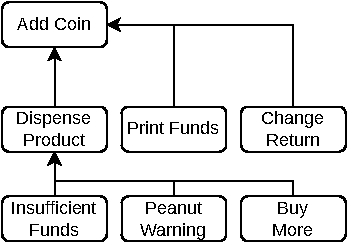
\includegraphics{figures/VendingMachine.pdf}
    \caption{Dependencies between Nim features.}
    \label{fig:nimDependencies}
\end{figure}

\subsubsection{Results}\label{sec:nim:results}
\pnote{Which pieces of data should I capture? Should I be looking to re-create the same table as Justin made for the vending machine?}\jnote{I think that would be good for now. I don't really think that dumping it to an FPGA really makes sense here. Maybe we can talk about how many lines of GraphVis each type of Nim creates?}

\subsection{SIMD Cache Coherence}\label{sec:cache}

\section{Future Work}
%%
%% The next two lines define the bibliography style to be used, and
%% the bibliography file.
\bibliographystyle{ACM-Reference-Format}
\bibliography{acmart,bibdbase,networks}

\end{document}
\endinput
%%
%% End of file `sample-sigplan.tex'.
